%%%%%%%%%%%%%%%%%%%%%%%%%%%%%%%%%%%%%%%%%%%%%%%%%%%%%%%%%%%%%%%%%%%%%%%%%%%%%
% Баталов Семен, 2021                                                       %
%%%%%%%%%%%%%%%%%%%%%%%%%%%%%%%%%%%%%%%%%%%%%%%%%%%%%%%%%%%%%%%%%%%%%%%%%%%%%

\documentclass[12pt, a4paper]{article}
\usepackage[left=2.5cm, right=2.5cm, top=2.5cm, bottom=2.5cm]{geometry}
\usepackage[utf8]{inputenc}
\usepackage{graphicx}
\graphicspath{{./pictures/}}
\usepackage[english, russian]{babel}
\usepackage{indentfirst}
\usepackage{misccorr}
\usepackage{amsmath}

\title{Кластеризация точек на плоскости}
\author{Баталов Семен}
\date{25.02.2021}

\begin{document}
    
    \sloppy
    
    \maketitle
    
    \section{Постановка задачи}
    
    Рассматривается плоскость, на которую случайным образом наносятся точки. 
    Нужно решить задачу кластеризации методом <<\textbf{K-Means++}>>. 
    Требуется показать конечный результат работы кластеризатора и оценить 
    расположение классов на этапе инициализации, сравнить результаты с 
    оригинальным разбиением на классы.
    
    Для написания программы использовался язык <<\textbf{Python}>>, подробнее 
    о ней можно узнать в папке <<\textbf{source}>> проекта.
    
    \section{K-Means и K-Means++}
    
    \subsection{K-Means}
    
    Алгоритм <<\textbf{K-Means}>> разбивает множество элементов векторного 
    пространства на заранее известное число кластеров <<k>>. В нашем случае 
    размерность пространства равна 2, а элементами являются точки, которые 
    описываются только двумя параметрами: абсциссой и ординатой.
    
    Основная идея заключается в том, что на каждой итерации перевычисляется 
    центр масс для каждого кластера, полученного на предыдущем шаге, затем 
    векторы разбиваются на кластеры вновь в соответствии с тем, какой из 
    новых центров оказался ближе по выбранной метрике.
    
    Алгоритм завершается, когда на какой-то итерации не происходит изменения 
    внутрикластерного расстояния. Это происходит за конечное число итераций, 
    так как количество возможных разбиений конечного множества конечно, а на 
    каждом шаге суммарное квадратичное отклонение уменьшается, поэтому 
    возникновение мертвого цикла невозможно.
    
    Важным этапом в алгоритме является первоначальная инициализация центров 
    классов. В <<\textbf{K-Means}>> центры выбираются случайно.
    
    \subsection{K-Means++}
    
    Алгоритм <<\textbf{K-Means++}>> ничем, кроме способа начальной 
    инициализации центров, не отличается от <<\textbf{K-Means}>>. В 
    <<\textbf{K-Means++}>> центры выбираются (как правило) удаленными друг от 
    друга, что с большей вероятностью приводит к лучшим результатам, чем 
    случайная инициализация.
    
    \section{Инструменты}
    
    Для работы была выбрана библиотека <<\textbf{sklearn}>>, из нее были 
    взяты алгоритмы <<\textbf{KMeans}>> и <<\textbf{kmeans\_plusplus}>>. 
    Первый из них осуществляет метод <<\textbf{K-Means}>>, второй генерирует 
    центры кластеров в соответствии с алгоритмом <<\textbf{K-Means++}>>.
    
    Для генерации случайных точек на плоскости использовались алгоритмы 
    библиотеки <<\textbf{sklearn}>>, а именно <<\textbf{make\_blobs}>>. Этот 
    алгоритм создает многоклассовые наборы данных, выделяя каждому классу 
    один или несколько нормально распределенных кластеров точек. 
    <<\textbf{make\_blobs}>> обеспечивает контроль относительно центров и 
    стандартных отклонений каждого кластера и используется для тестирования 
    алгоритмов кластеризации.
    
    \section{Результаты}
    
    В экспериментах варьировалось количество точек на плоскости, количество 
    кластеров, коэффициенты, отвечающие за распределение точек по плоскости. 
    
    Основной задачей было показать конечный результат работы кластеризатора и 
    в случае <<\textbf{K-Means++}>> оценить расположение классов, используя 
    начальную инициализацию центров, сравнить результаты с оригинальным 
    разбиением на классы.
    
    В целом, кластеризаторы <<\textbf{K-Means}>> и <<\textbf{K-Means++}>> 
    работают корректно. Стоит отметить, что начальная инициализация (центров 
    кластеров) во втором алгоритме позволяет с самого начала равномернее 
    распределить центры кластеров по множеству точек, во всех примерах это 
    отчетливо прослеживается. Также видно, что результаты работы обоих 
    кластеризаторов (для оределенного множества) слабо отличаются друг от 
    друга, то есть конечные положения центров кластеров во многих примерах 
    совпадают, а в остальных различие незначительно. Можно сделать вывод, что 
    начальные условия (на положения центров кластеров) при данной постановке 
    задачи если и оказывают влияние на конечный результат, то незначительное.
    
    Важно отметить, что в некоторых примерах (Рис.~\ref{image2}), 
    (Рис.~\ref{image5}) результаты работы алгоритмов не совпадали с истинным 
    разбиением множества на кластеры. Это объясняется возникновением плотных 
    областей пересечения нескольких кластеров, в которых сконцентрировано 
    столько точек, что программа считает их отдельными классами. В то же 
    время примеры (Рис.~\ref{image1}), (Рис.~\ref{image3}), 
    (Рис.~\ref{image4}) демонстрируют корректную работу классификаторов. Все 
    тестовые множества и результаты работы алгоритмов представлены ниже.
    
    \begin{figure} [h]
        \center{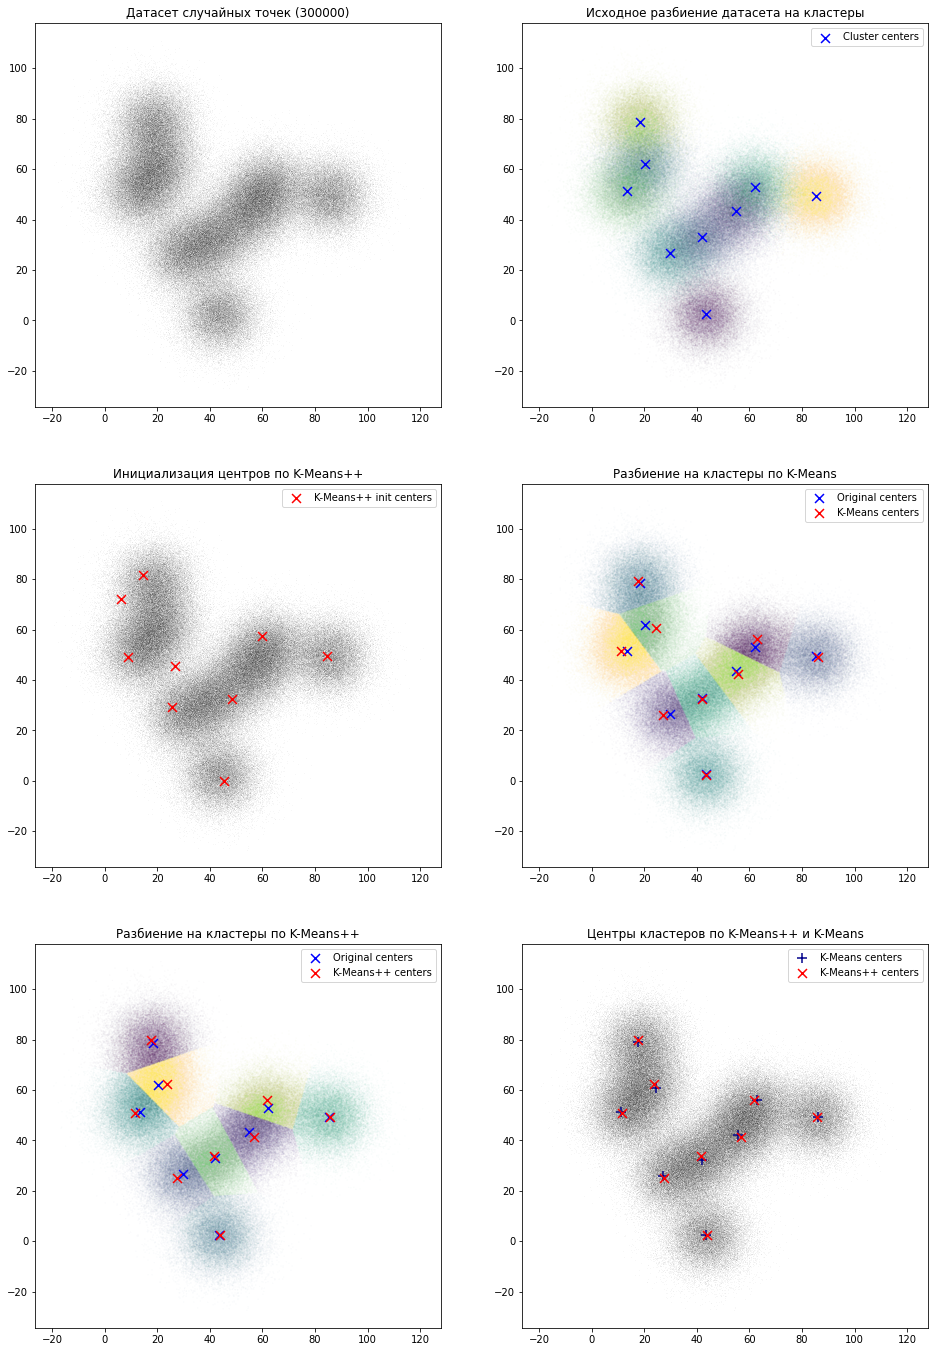
\includegraphics[width = \textwidth]{9_300_2_analysis.png}}
        \caption{9 кластеров, 300000 точек}
        \label{image1}
    \end{figure}
    
    \begin{figure} [h]
        \center{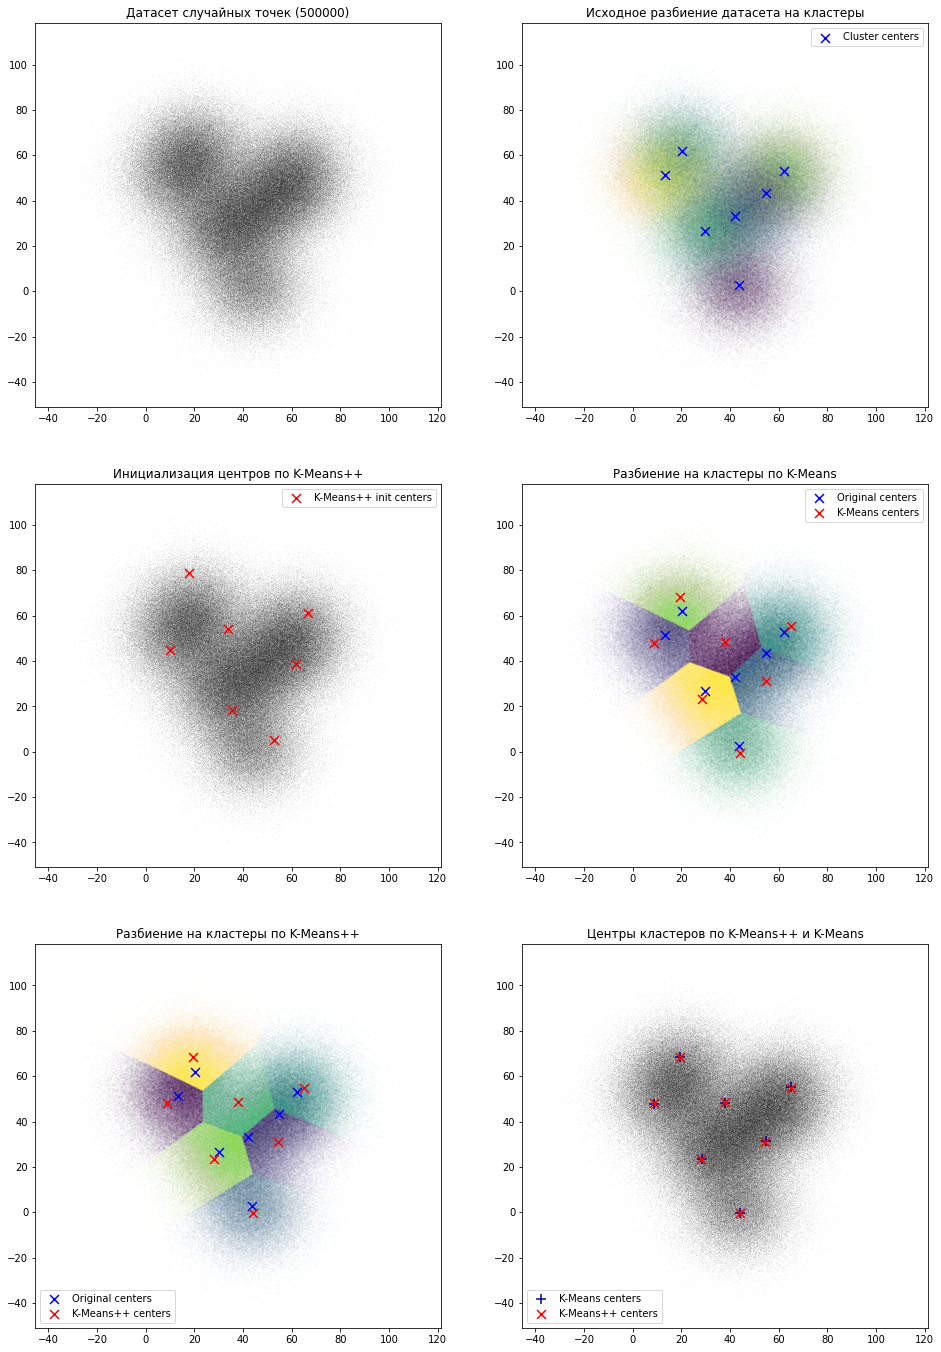
\includegraphics[width = \textwidth]{7_500_2_analysis.png}}
        \caption{7 кластеров, 500000 точек}
        \label{image2}
    \end{figure}
    
    \begin{figure} [h]
        \center{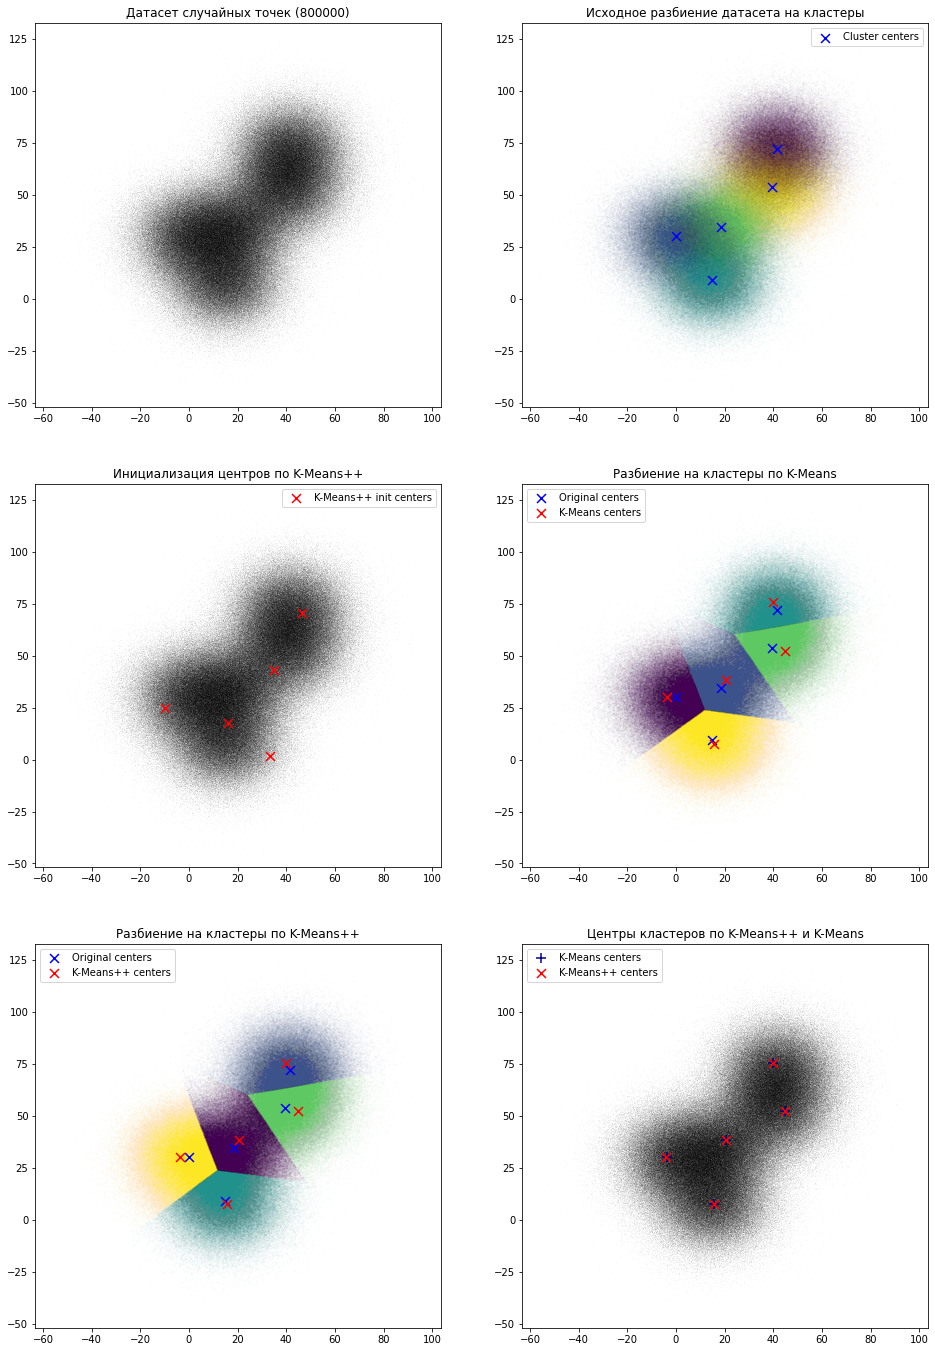
\includegraphics[width = \textwidth]{5_800_2_analysis.png}}
        \caption{5 кластеров, 800000 точек}
        \label{image3}
    \end{figure}
    
    \begin{figure} [h]
        \center{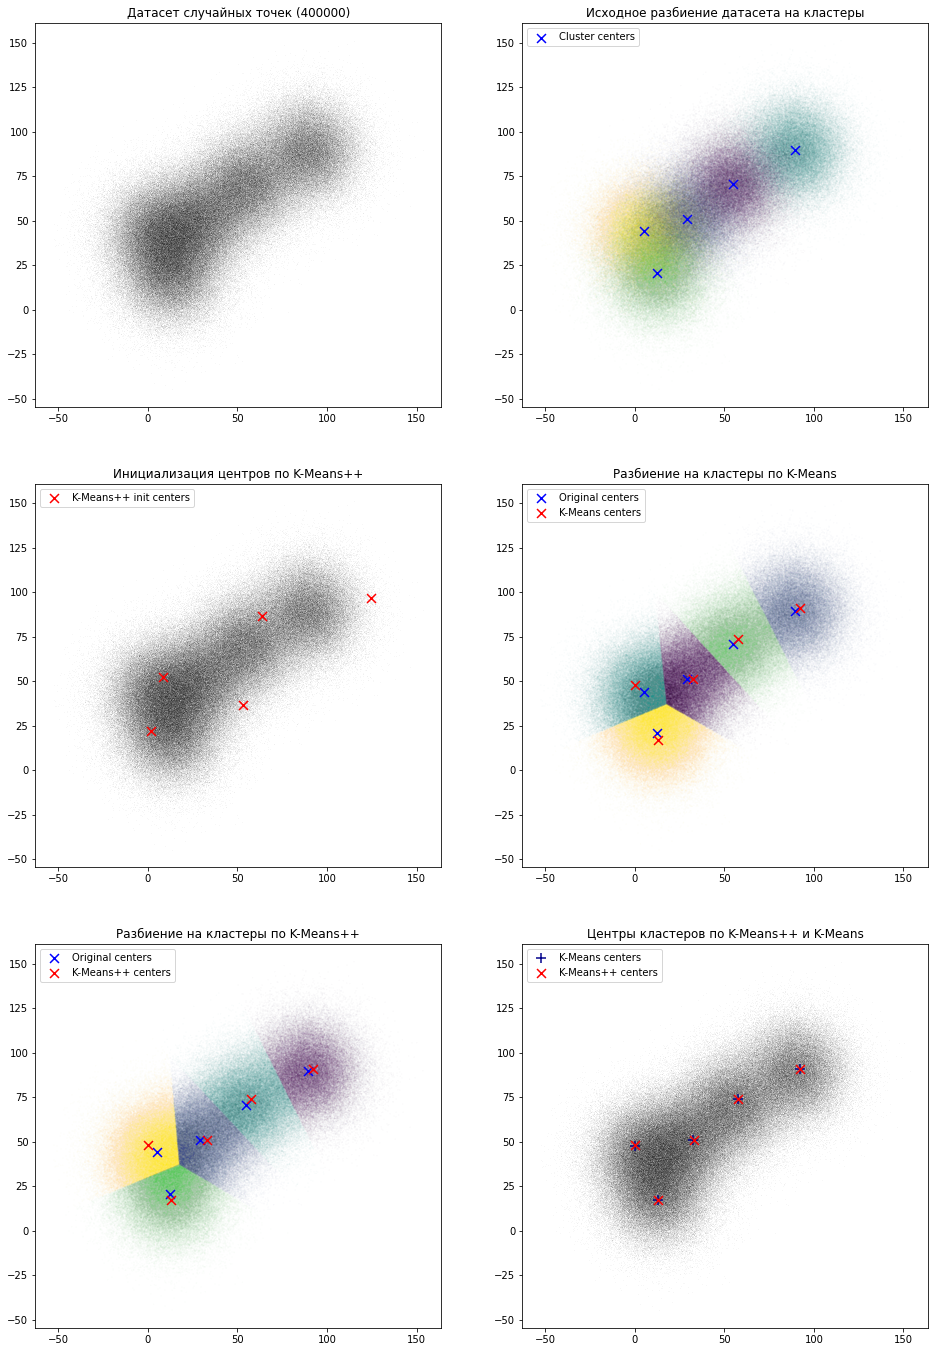
\includegraphics[width = \textwidth]{5_400_3_analysis.png}}
        \caption{5 кластеров, 400000 точек}
        \label{image4}
    \end{figure}
    
    \begin{figure} [h]
        \center{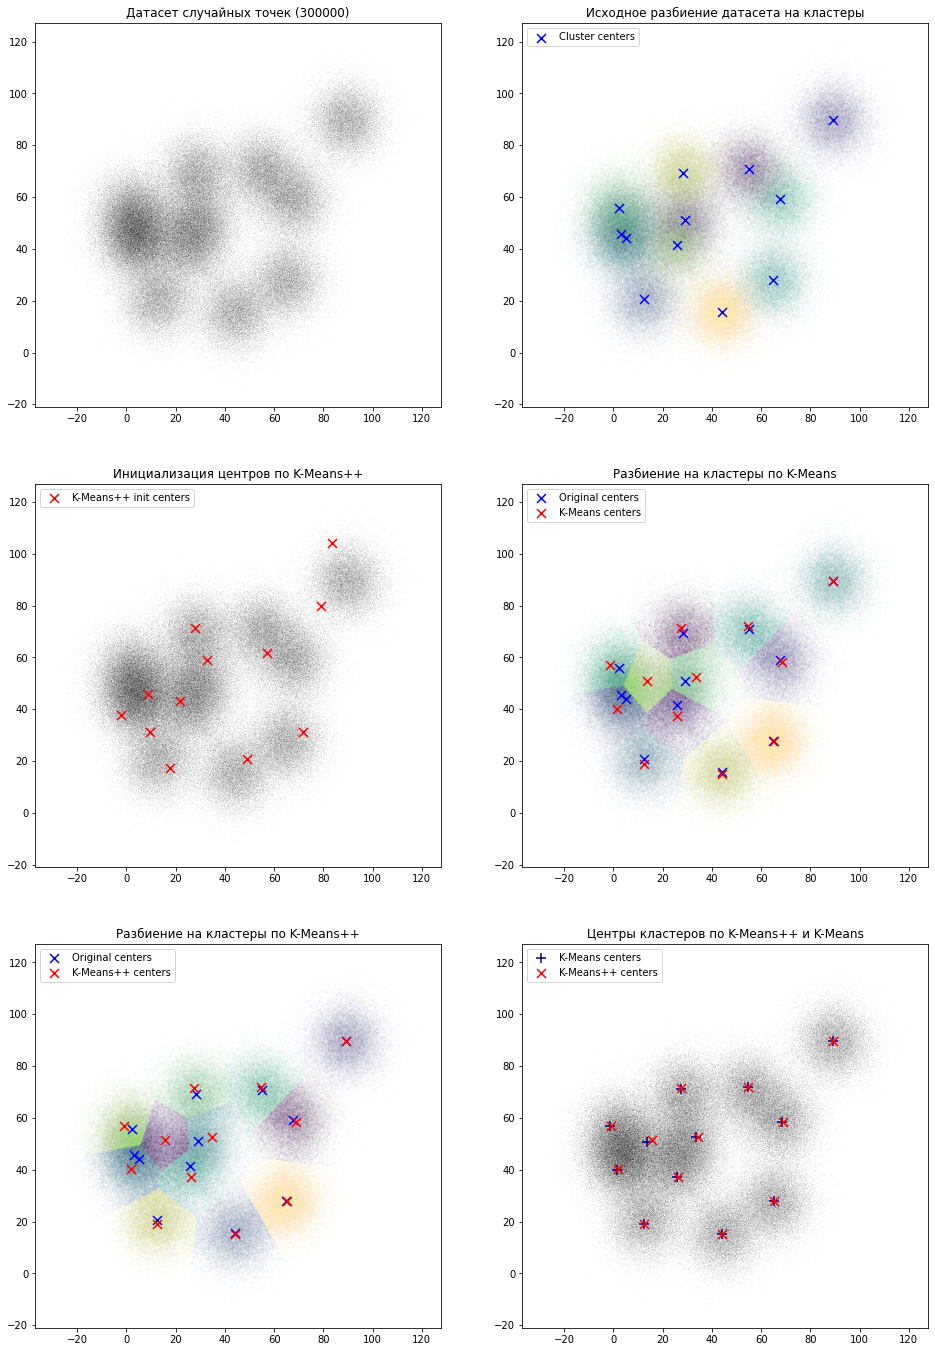
\includegraphics[width = \textwidth]{12_400_3_analysis.png}}
        \caption{12 кластеров, 400000 точек}
        \label{image5}
    \end{figure}
    
\end{document}